\documentclass[10pt]{beamer}
\usepackage{../../../resources/themes/algolymp-dense}
\usepackage{booktabs}
\usepackage{amssymb}
\usepackage{tikz}
\usetikzlibrary{positioning, calc, patterns}

\title{Indicatorul lui Euler.\\Principiul Includerii și al Excluderii}
\subtitle{Bonus: Funcția Möbius}
\author{Andrei Mihai Ciobanu}
\institute{Algolymp Summer School}
\date{}
\titlegraphic{\includegraphics[width=3cm]{../../../resources/algolymp-logo.png}}
\setbeamertemplate{frame footer}{Algolymp Summer School}

\begin{document}

\begin{frame}
  \titlepage
\end{frame}

\begin{frame}{Cuprins}
  \tableofcontents
\end{frame}

%% ============================================================
\section{Indicatorul lui Euler}
%% ============================================================

\begin{frame}{Definiție}
  \begin{block}{Indicatorul lui Euler \textemdash{} $\varphi(n)$}
    $\varphi(n)$ = numărul de numere întregi $k$ \textbf{coprime} cu $n$ (adică $\gcd(k, n) = 1$) din intervalul $[1, n]$.
  \end{block}
  \smallskip
  \textbf{Exemple directe:}
  \begin{itemize}\itemsep2pt
    \item $\varphi(1) = 1$ \textemdash{} prin convenție, $\gcd(1,1)=1$
    \item $\varphi(5) = 4$ \textemdash{} 5 e prim, $1, 2, 3, 4$ sunt coprime cu 5
    \item $\varphi(6) = 2$ \textemdash{} doar $1$ și $5$ sunt coprime cu 6
    \item $\varphi(12) = 4$ \textemdash{} $1, 5, 7, 11$ sunt coprime cu 12
    \item $\varphi(p) = p-1$ pentru orice $p$ prim
  \end{itemize}
\end{frame}

\begin{frame}{Exemplu vizual \textemdash{} $\varphi(12) = 4$}
  $12 = 2^2 \cdot 3$ \textemdash{} un număr $k$ nu este coprime cu 12 dacă e multiplu de 2 sau de 3.
  \begin{center}
  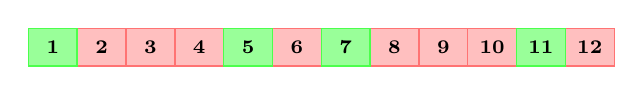
\begin{tikzpicture}
    \def\cw{0.62}
    \def\ch{0.48}
    \foreach \i in {2,3,4,6,8,9,10,12} {
      \filldraw[fill=red!25, draw=red!55, line width=0.5pt]
        (\i*\cw-\cw, 0) rectangle (\i*\cw, \ch);
    }
    \foreach \i in {1,5,7,11} {
      \filldraw[fill=green!40, draw=green!70, line width=0.5pt]
        (\i*\cw-\cw, 0) rectangle (\i*\cw, \ch);
    }
    \foreach \i in {1,...,12} {
      \node[font=\scriptsize\bfseries] at (\i*\cw-0.5*\cw, 0.5*\ch) {\i};
    }
  \end{tikzpicture}
  \end{center}
  \begin{columns}[T]
    \begin{column}{0.48\textwidth}
      \textcolor{green!60!black}{\rule{0.8em}{0.8em}} coprime cu 12: $\{1, 5, 7, 11\}$ \textemdash{} 4 numere
    \end{column}
    \begin{column}{0.48\textwidth}
      \textcolor{red!60!black}{\rule{0.8em}{0.8em}} nu sunt coprime: mulțipli de 2 sau 3
    \end{column}
  \end{columns}
  \medskip
  Verificăm: $\gcd(5, 12)=1$, $\gcd(7, 12)=1$, $\gcd(11, 12)=1$. Deci $\varphi(12) = 4$.
\end{frame}

\begin{frame}{Proprietăți fundamentale}
  \begin{block}{1. $\varphi$ pentru puteri de prime}
    \[
      \varphi(p^k) = p^k - p^{k-1} = p^{k-1}(p-1) = p^k \cdot \frac{p-1}{p}
    \]
    \textbf{Demonstrație:} din $\{1, \ldots, p^k\}$, numerele care nu sunt coprime
    cu $p^k$ sunt exact multiplii lui $p$: $p,\, 2p,\, \ldots,\, p^{k-1} \cdot p$
    \textemdash{} adică $p^{k-1}$ numere.
    Deci $\varphi(p^k) = p^k - p^{k-1}$.
    \smallskip

    \textbf{Exemple:}
    \begin{itemize}\itemsep1pt
      \item $\varphi(4) = \varphi(2^2) = 4 \cdot \frac{1}{2} = 2$
      \item $\varphi(8) = \varphi(2^3) = 8 \cdot \frac{1}{2} = 4$
      \item $\varphi(9) = \varphi(3^2) = 9 \cdot \frac{2}{3} = 6$
    \end{itemize}
  \end{block}
  \smallskip
  \begin{block}{2. Multiplicativitate}
    Dacă $\gcd(m, n) = 1$, atunci $\varphi(mn) = \varphi(m) \cdot \varphi(n)$.
  \end{block}
\end{frame}

\begin{frame}{Formula generală pentru $\varphi(n)$}
  Fie $n = p_1^{a_1} \cdot p_2^{a_2} \cdots p_k^{a_k}$ factorizarea lui $n$.
  \begin{block}{Formula produsului}
    \[
      \varphi(n) = n \cdot \prod_{p \mid n,\; p \text{ prim}} \!\!\left(1 - \frac{1}{p}\right)
    \]
  \end{block}
  \smallskip
  \textbf{Derivare:} aplicăm multiplicativitatea, apoi formula pentru puteri de prime:
  \[
    \varphi(n)
    = \prod_{i=1}^k \varphi(p_i^{a_i})
    = \prod_{i=1}^k p_i^{a_i} \cdot \frac{p_i-1}{p_i}
    = \underbrace{\prod_{i=1}^k p_i^{a_i}}_{=\,n}
      \cdot \prod_{i=1}^k \frac{p_i-1}{p_i}
    = n \cdot \prod_{i=1}^k \!\left(1 - \tfrac{1}{p_i}\right)
  \]
  \smallskip
  \textbf{Exemplu numeric:} $n = 12 = 2^2 \cdot 3$
  \[
    \varphi(12) = 12 \cdot \left(1 - \tfrac{1}{2}\right)\!\left(1 - \tfrac{1}{3}\right)
    = 12 \cdot \tfrac{1}{2} \cdot \tfrac{2}{3} = 4
  \]
\end{frame}

\begin{frame}[fragile]{Cum aflăm $\varphi(n)$}
  \textbf{Idee:} factorizăm $n$ și aplicăm formula. Complexitate: $O(\sqrt{n})$.
  \begin{lstlisting}
long long phi(long long n) {
    long long result = n;
    for (long long p = 2; p * p <= n; p++) {
        if (n % p == 0) {
            while (n % p == 0) {
                n /= p;
            }
            result -= result / p;
        }
    }
    if (n > 1) {
        result -= result / n;
    }
    return result;
}
  \end{lstlisting}
  La fiecare pas cu prim $p$ aplicăm $\mathtt{result} \mathrel{*}= (1 - 1/p)$,
  adică $\mathtt{result} \mathrel{-}= \mathtt{result}/p$.
\end{frame}

\begin{frame}[fragile]{Ciur pentru $\varphi(i)$, $i \in [1, N]$ \textemdash{} $O(N \log N)$}
  \textbf{Idee:} analog cu Ciurul lui Eratostene. Inițializăm $\varphi[i] = i$,
  apoi pentru fiecare prim $p$ actualizăm toți multiplii aplicând $\times(1-1/p)$.
  \begin{lstlisting}
const int nmax = 1000000;
int phi[nmax + 1];

void sieve_phi(int n) {
    for (int i = 0; i <= n; i++) {
        phi[i] = i;
    }
    for (int i = 2; i <= n; i++) {
        if (phi[i] == i) {
            for (int j = i; j <= n; j += i) {
                phi[j] -= phi[j] / i;
            }
        }
    }
}
  \end{lstlisting}
  \beginnote{Complexitatea reală este $O(N \log \log N)$ (suma armonică a numerelor prime),
  dar folosim $O(N \log N)$ pentru simplitate.}
\end{frame}

\begin{frame}{Identitatea sumei}
  \begin{block}{Proprietate}
    \[
      \sum_{d \mid n} \varphi(d) = n
    \]
  \end{block}
  \smallskip
  \textbf{Exemplu:} $n = 6$, divizorii sunt $1, 2, 3, 6$:
  \[
    \varphi(1)+\varphi(2)+\varphi(3)+\varphi(6) = 1+1+2+2 = 6 \checkmark
  \]
\end{frame}

\begin{frame}[fragile]{Aplicație \textemdash{} \href{https://www.infoarena.ro/problema/fractii}{fractii} \textcolor{gray}{(infoarena)}}
  \textbf{Problemă:} Dat $N$, numărați fracțiile ireductibile $\frac{p}{q}$
  cu $1 \leq p, q \leq N$ ($\gcd(p,q) = 1$).
  \begin{itemize}\itemsep3pt
    \item \textbf{$p = q$:} $\gcd(p, p) = p = 1$ doar pentru $p = 1$
      $\Rightarrow$ fracția $\frac{1}{1}$, \textbf{1 fracție}
    \item \textbf{$p \neq q$:} fracțiile vin în perechi
      $\frac{p}{q} \leftrightarrow \frac{q}{p}$ (subunitară $\leftrightarrow$ supraunitară),
      ambele ireductibile sau niciuna.
      Numărăm \textbf{supraunitarele} ($p > q$): pentru fiecare numărător $p \in [2, N]$,
      numitorii $q \in [1, p-1]$ coprimi cu $p$ sunt exact $\varphi(p)$.
  \end{itemize}
  \[
    \text{Răspuns}
    = \underbrace{1}_{\frac{1}{1}}
    + \underbrace{2 \cdot \sum_{p=2}^{N} \varphi(p)}_{\text{sub- + supraunitare}}
    = 2\sum_{p=1}^{N} \varphi(p) - 1
  \]
  \begin{lstlisting}
long long solve(int n) {
    long long ans = 0;
    for (int p = 1; p <= n; p++) {
        ans += phi[p];
    }
    return 2 * ans - 1;
}
  \end{lstlisting}
\end{frame}

%% ============================================================
\section{Principiul Includerii și Excluderii}
%% ============================================================

\begin{frame}{Motivație \textemdash{} Numărarea cu condiții multiple}
  \textbf{Problemă:} Câte numere din $[1, 100]$ sunt divizibile cu 2 \textbf{sau} cu 3?
  \smallskip

  \textbf{Greșit:} $\lfloor 100/2 \rfloor + \lfloor 100/3 \rfloor = 50 + 33 = 83$
  \textemdash{} am numărat de două ori numerele divizibile cu $2 \cdot 3 = 6$!
  \smallskip

  \textbf{Corect:}
  \[
    \underbrace{\lfloor 100/2 \rfloor}_{=50}
    + \underbrace{\lfloor 100/3 \rfloor}_{=33}
    - \underbrace{\lfloor 100/6 \rfloor}_{=16}
    = 67
  \]
  \smallskip
  Aceasta este esența \textbf{Principiului Includerii și Excluderii (pinex)}:
  adunăm, scădem, adunăm $\ldots$ până numărăm fiecare element exact o dată.
\end{frame}

\begin{frame}{Pinex \textemdash{} 2 mulțimi}
  \begin{columns}[T]
    \begin{column}{0.45\textwidth}
      \begin{center}
      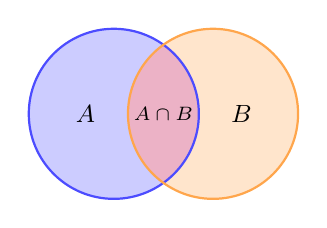
\begin{tikzpicture}[scale=0.9]
        \fill[blue!20] (-0.7,0) circle (1.2);
        \fill[orange!20] (0.7,0) circle (1.2);
        \begin{scope}
          \clip (-0.7,0) circle (1.2);
          \fill[purple!30] (0.7,0) circle (1.2);
        \end{scope}
        \draw[blue!70, thick] (-0.7,0) circle (1.2);
        \draw[orange!70, thick] (0.7,0) circle (1.2);
        \node[font=\small] at (-1.1, 0) {$A$};
        \node[font=\small] at (1.1, 0) {$B$};
        \node[font=\scriptsize] at (0, 0) {$A\cap B$};
      \end{tikzpicture}
      \end{center}
    \end{column}
    \begin{column}{0.52\textwidth}
      \begin{block}{Formula pentru 2 mulțimi}
        \[
          |A \cup B| = |A| + |B| - |A \cap B|
        \]
      \end{block}
      \smallskip
      De ce? Elementele din $A \cap B$ sunt adăugate de două ori la $|A|+|B|$,
      deci le scădem o dată.
    \end{column}
  \end{columns}
  \smallskip
  \textbf{Exemplu:} Câte din $[1,30]$ sunt div cu 2 sau 5?
  \[
    \lfloor 30/2 \rfloor + \lfloor 30/5 \rfloor - \lfloor 30/10 \rfloor
    = 15 + 6 - 3 = 18
  \]
\end{frame}

\begin{frame}{Pinex \textemdash{} 3 mulțimi}
  \begin{columns}[T]
    \begin{column}{0.44\textwidth}
      \begin{center}
        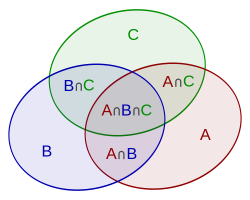
\includegraphics[width=\linewidth]{Inclusion-exclusion.png}
      \end{center}
    \end{column}
    \begin{column}{0.53\textwidth}
      \begin{block}{Formula pentru 3 mulțimi}
        \begin{align*}
          |A \cup B \cup C| &= |A| + |B| + |C| \\
            &- |A\cap B| - |A\cap C| - |B\cap C| \\
            &+ |A\cap B\cap C|
        \end{align*}
      \end{block}
      \smallskip
      \textbf{Logică:}
      \begin{itemize}\itemsep1pt\footnotesize
        \item Elementele din exact 2 mulțimi: adăugate de 2 ori, scăzute o dată $\Rightarrow$ numărate corect
        \item Elementele din toate 3: adăugate 3 ori, scăzute 3 ori, adăugate 1 dată $\Rightarrow$ corect
      \end{itemize}
    \end{column}
  \end{columns}
\end{frame}

\begin{frame}{Pinex \textemdash{} Formula generală}
  \begin{block}{Formula generală pentru $n$ mulțimi}
    \[
      \left|\bigcup_{i=1}^{n}A_{i}\right|
      =\sum_{i=1}^{n}|A_{i}|
      -\!\!\sum_{1\leq i<j\leq n}\!\!|A_{i}\cap A_{j}|
      +\!\!\sum_{1\leq i<j<k\leq n}\!\!|A_{i}\cap A_{j}\cap A_{k}|
      -\cdots
      +(-1)^{n+1}\left|A_{1}\cap\cdots\cap A_{n}\right|
    \]
  \end{block}
  \smallskip
  \textbf{Semne alternante:} adunăm intersecțiile de dimensiune impară,
  scădem cele de dimensiune pară.
  \begin{center}
  {\small
  \begin{tabular}{c|c|l}
    \toprule
    Dimensiune & Semn & \\
    \midrule
    1 & $+$ & sumele individuale $|A_i|$ \\
    2 & $-$ & scădem intersecțiile perechi \\
    3 & $+$ & adunăm intersecțiile triple \\
    $\vdots$ & $\vdots$ & \\
    $n$ & $(-1)^{n+1}$ & \\
    \bottomrule
  \end{tabular}}
  \end{center}
  \textbf{Complexitate:} $O(2^n)$ termeni. Eficient pentru $n \leq 20$.
\end{frame}

\begin{frame}{Pinex $\Rightarrow$ Indicatorul lui Euler}
  Fie $n = p_1^{a_1} \cdots p_k^{a_k}$. Definim:
  \begin{block}{}
    $A_{p_i} = \{\,m \in [1, n] : p_i \mid m\,\}$ \textemdash{} multiplii lui $p_i$ din $[1, n]$
  \end{block}
  \smallskip
  \begin{columns}[T]
    \begin{column}{0.48\textwidth}
      \textbf{Proprietăți cheie:}
      \begin{itemize}\itemsep2pt
        \item $|A_{p_i}| = \dfrac{n}{p_i}$ \quad (exact, deoarece $p_i \mid n$)
        \item $A_{p_i} \cap A_{p_j}$ = multiplii lui $p_i p_j$, deci $|A_{p_i} \cap A_{p_j}| = \dfrac{n}{p_i p_j}$
        \item În general: $\left|\bigcap_{i \in S} A_{p_i}\right| = \dfrac{n}{\prod_{i \in S} p_i}$
      \end{itemize}
    \end{column}
    \begin{column}{0.48\textwidth}
      \textbf{Exemplu:} $n = 30 = 2 \cdot 3 \cdot 5$
      \begin{itemize}\itemsep2pt
        \item $A_2 = \{2,4,6,\ldots,30\}$ \quad $|A_2| = 15$
        \item $A_3 = \{3,6,9,\ldots,30\}$ \quad $|A_3| = 10$
        \item $A_5 = \{5,10,15,\ldots,30\}$ \quad $|A_5| = 6$
      \end{itemize}
      \smallskip
      $\varphi(30)$ = numerele din $[1,30]$ care \textbf{nu} sunt în niciun $A_{p_i}$
    \end{column}
  \end{columns}
\end{frame}

\begin{frame}{Pinex $\Rightarrow$ Indicatorul lui Euler}
  Aplicăm pinex pe $A_{p_1}, \ldots, A_{p_k}$:
  \[
    \varphi(n) = n - \left|\bigcup_{i=1}^k A_{p_i}\right|
    = n - \sum_i \frac{n}{p_i} + \sum_{i<j} \frac{n}{p_ip_j} - \cdots
  \]
  Scoatem $n$ factor comun:
  \[
    \varphi(n) = n\!\left(1 - \sum_i \frac{1}{p_i} + \sum_{i<j} \frac{1}{p_ip_j} - \cdots\right)
  \]
  Analizăm termenii pentru un $k$ mic \textemdash{} exemplu $k=2$:
  \begin{block}{}
    \vspace{-4pt}
    \[
      n\!\left(1 - \tfrac{1}{p_1} - \tfrac{1}{p_2} + \tfrac{1}{p_1 p_2}\right)
      = n\!\left(1 - \tfrac{1}{p_1}\right)\!\left(1 - \tfrac{1}{p_2}\right) \checkmark
    \]
    \vspace{-6pt}
  \end{block}
  \vspace{-2pt}
  În general: $\displaystyle\varphi(n) = n \prod_{i=1}^k \!\left(1 - \frac{1}{p_i}\right)$
\end{frame}

\begin{frame}{Aplicație \textemdash{} Câte numere $\leq N$ sunt coprime cu $M$?}
  \textbf{Problemă:} Dat $N$ și $M$, numărați $k \in [1, N]$ cu $\gcd(k, M) = 1$.

  \textbf{Algoritm:}
  \begin{enumerate}\itemsep2pt
    \item Factorizăm $M$ $\Rightarrow$ obținem primii distincți $p_1, \ldots, p_t$
    \item Definim $A_{p_i} = \{k \leq N : p_i \mid k\}$, $|A_{p_i}| = \lfloor N/p_i \rfloor$
    \item Aplicăm pinex cu bitmask pe toate subseturile ai $\{p_1, \ldots, p_t\}$
  \end{enumerate}
  \smallskip
  \textbf{Exemplu:} $N = 30$, $M = 12 = 2^2 \cdot 3$, deci $\{p_1, p_2\} = \{2, 3\}$:
  \[
    \lfloor 30/1 \rfloor - \lfloor 30/2 \rfloor - \lfloor 30/3 \rfloor + \lfloor 30/6 \rfloor
    = 30 - 15 - 10 + 5 = 10
  \]
  Verificare: $\varphi(12)/12 \cdot 30 = 4/12 \cdot 30 = 10$. \checkmark
\end{frame}

\begin{frame}[fragile]{Implementare pinex cu măști de biți}
  \begin{lstlisting}
// p[] = factorii primi distincti ai lui M
long long count_coprime(long long N, vector<long long>& p) {
    int k = p.size();
    long long result = 0;
    for (int mask = 0; mask < (1 << k); mask++) {
        int bits = 0;
        long long prod = 1;
        for (int i = 0; i < k; i++) {
            if (mask & (1 << i)) {
                bits++;
                prod *= p[i];
            }
        }
        if (bits % 2 == 0) {
            result += N / prod;
        } else {
            result -= N / prod;
        }
    }
    return result;
}
  \end{lstlisting}
  \textbf{Obs:} \texttt{mask = 0} contribuie $+N$ (submulțimea vidă, semn $+$).
\end{frame}


%% ============================================================
\section{Funcția Möbius}
%% ============================================================

\begin{frame}{Funcția Möbius \textemdash{} Definiție}
  \begin{block}{Funcția $\mu(n)$}
    \[
      \mu(n) = \begin{cases}
        1 & \text{dacă } n = 1 \\
        0 & \text{dacă } n \text{ are un factor pătratic} \\
        (-1)^k & \text{dacă } n = p_1 p_2 \cdots p_k \text{ (prime distincte)}
      \end{cases}
    \]
  \end{block}
  \smallskip
  Cu alte cuvinte: $\mu(n) = 0$ dacă există $p$ prim cu $p^2 \mid n$;
  altfel $\mu(n) = (-1)^{\omega(n)}$, unde $\omega(n)$ e numărul de factori
  primi distincți ai lui $n$.
  \smallskip

  \textbf{Observație:} $\mu$ este multiplicativă: $\gcd(m,n)=1 \Rightarrow \mu(mn) = \mu(m)\mu(n)$.
\end{frame}

\begin{frame}{Tabelul $\mu(n)$ pentru $n = 1 \ldots 20$}
  \begin{columns}[T]
    \begin{column}{0.48\textwidth}
      \begin{center}{\small
      \begin{tabular}{c|l|r}
        \toprule
        $n$ & Factorizare & $\mu(n)$ \\
        \midrule
        1  & $1$                 & $1$  \\
        2  & $2$                 & $-1$ \\
        3  & $3$                 & $-1$ \\
        4  & $2^2$               & $0$  \\
        5  & $5$                 & $-1$ \\
        6  & $2 \cdot 3$         & $1$  \\
        7  & $7$                 & $-1$ \\
        8  & $2^3$               & $0$  \\
        9  & $3^2$               & $0$  \\
        10 & $2 \cdot 5$         & $1$  \\
        \bottomrule
      \end{tabular}}
      \end{center}
    \end{column}
    \begin{column}{0.48\textwidth}
      \begin{center}{\small
      \begin{tabular}{c|l|r}
        \toprule
        $n$ & Factorizare & $\mu(n)$ \\
        \midrule
        11 & $11$                & $-1$ \\
        12 & $2^2 \cdot 3$       & $0$  \\
        13 & $13$                & $-1$ \\
        14 & $2 \cdot 7$         & $1$  \\
        15 & $3 \cdot 5$         & $1$  \\
        16 & $2^4$               & $0$  \\
        17 & $17$                & $-1$ \\
        18 & $2 \cdot 3^2$       & $0$  \\
        19 & $19$                & $-1$ \\
        20 & $2^2 \cdot 5$       & $0$  \\
        \bottomrule
      \end{tabular}}
      \end{center}
    \end{column}
  \end{columns}
\end{frame}

\begin{frame}{Proprietatea fundamentală a lui $\mu$}
  \begin{block}{Suma $\mu$ pe divizori}
    \[
      \sum_{d \mid n} \mu(d) = [n = 1] =
      \begin{cases} 1 & \text{dacă } n = 1 \\ 0 & \text{dacă } n > 1 \end{cases}
    \]
  \end{block}
  \smallskip
  \textbf{Exemplu:} $n = 6$, divizorii sunt $1, 2, 3, 6$:
  \[
    \mu(1) + \mu(2) + \mu(3) + \mu(6) = 1 + (-1) + (-1) + 1 = 0 \checkmark
  \]
  \textbf{Intuiție:} contribuțiile pozitive și negative se anulează exact
  pentru orice $n > 1$ cu cel puțin un factor prim.
\end{frame}

\begin{frame}{Inversiunea Möbius \textemdash{} \textcolor{red}{\textsl{Topic avansat}}}
  \begin{block}{Teorema inversiunii Möbius}
    Dacă $f$ și $g$ sunt funcții definite pe $\mathbb{N}^*$ cu:
    \[
      g(n) = \sum_{d \mid n} f(d)
    \]
    atunci:
    \[
      f(n) = \sum_{d \mid n} \mu\!\left(\frac{n}{d}\right) g(d)
      = \sum_{d \mid n} \mu(d) \, g\!\left(\frac{n}{d}\right)
    \]
  \end{block}
  \smallskip
  \textbf{Lectură recomandată:}
  \href{https://codeforces.com/blog/entry/53925}{\textit{Codeforces blog \#53925}}
  \textemdash{} prezintă cum calculăm numărul de perechi coprime din $[1,n]$
  și suma $\gcd$-urilor tuturor perechilor din $[1,n]$ folosind inversiunea Möbius.
\end{frame}


\begin{frame}[fragile]{Ciur pentru $\mu(i)$, $i \in [1, N]$ \textemdash{} $O(N \log N)$}
  \textbf{Idee:} similar cu ciurul pentru $\varphi$. Fiecare prim $p$ aplică
  factorul $(-1)$ la toți multiplii; multiplii lui $p^2$ devin 0.
  \begin{lstlisting}
// Global: const int nmax = 1000000; int mu[nmax + 1]; bool priem[nmax + 1];
void sieve_mobius(int n) {
    for (int i = 1; i <= n; i++) {
        mu[i] = prime[i] = 1;
    }
    for (int i = 2; i <= n; i++) {
        if (prime[i]) {
            for (int j = i; j <= n; j += i) {
                if (j != i) {
                    prime[j] = false;
                }
                mu[j] *= -1;
                if ((j / i) % i == 0) {
                    mu[j] = 0;
                }
            }
        }
    }
}
  \end{lstlisting}
\end{frame}

%% ============================================================
\section{Recapitulare}
%% ============================================================

\begin{frame}{Probleme \textemdash{} Indicatorul lui Euler}
  \begin{enumerate}\itemsep3pt\normalsize
    \item \href{https://www.pbinfo.ro/probleme/2608/biprime}{\textbf{biPrime}}
          \textcolor{gray}{(pbinfo \#2608)}
    \item \href{https://www.infoarena.ro/problema/fractii}{\textbf{fractii}}
          \textcolor{gray}{(infoarena)}
    \item \href{https://www.pbinfo.ro/probleme/3047/fibofrac}{\textbf{fiboFrac}}
          \textcolor{gray}{(pbinfo \#3047)}
    \item \href{https://www.pbinfo.ro/probleme/3289/maxprimeintreele}{\textbf{maxprimeintreele}}
          \textcolor{gray}{(pbinfo \#3289)}
    \item \href{https://www.pbinfo.ro/probleme/3227/tramvaie}{\textbf{tramvaie}}
          \textcolor{gray}{(pbinfo \#3227)}
  \end{enumerate}
\end{frame}

\begin{frame}{Probleme \textemdash{} Pinex}
  \begin{enumerate}\itemsep3pt\normalsize
    \item \href{https://www.infoarena.ro/problema/pinex}{\textbf{pinex}}
          \textcolor{gray}{(infoarena)}
    \item \href{https://kilonova.ro/problems/1546}{\textbf{pro3}}
          \textcolor{gray}{(Kilonova \#1546)}
    \item \href{https://www.infoarena.ro/problema/reuniune}{\textbf{Reuniune}}
          \textcolor{gray}{(infoarena)}
    \item \href{https://kilonova.ro/problems/3394}{\textbf{Nice Compatibility}}
          \textcolor{gray}{(Kilonova \#3394)}
  \end{enumerate}
\end{frame}

\begin{frame}{Resurse}
  \begin{enumerate}\itemsep3pt\normalsize
    \item \href{https://www.pbinfo.ro/articole/18882/indicatorul-lui-euler}%
          {\textbf{pbinfo} \textemdash{} Indicatorul lui Euler}
    \item \href{https://cp-algorithms.com/algebra/phi-function.html}%
          {\textbf{CP-Algorithms} \textemdash{} Euler's totient function}
    \item \href{https://en.wikipedia.org/wiki/Euler\%27s_totient_function}%
          {\textbf{Wikipedia} \textemdash{} Euler's totient function}
    \item \href{https://cp-algorithms.com/combinatorics/inclusion-exclusion.html}%
          {\textbf{CP-Algorithms} \textemdash{} The Inclusion-Exclusion Principle}
    \item \href{https://usaco.guide/plat/PIE?lang=cpp}%
          {\textbf{USACO Guide} \textemdash{} Inclusion-Exclusion Principle}
    \item \href{https://en.wikipedia.org/wiki/M\%C3\%B6bius_function}%
          {\textbf{Wikipedia} \textemdash{} Möbius function}
    \item \href{https://codeforces.com/blog/entry/53925}%
          {\textbf{Codeforces} \textemdash{} [Tutorial] Math note \textemdash{} Möbius inversion}
  \end{enumerate}
\end{frame}

\end{document}
